\documentclass[10pt]{article}

\usepackage{mathtools, amssymb, bm}
\usepackage{microtype}
\usepackage[utf8]{inputenc}
\usepackage[margin = 0.75in]{geometry}
\usepackage{booktabs}
\usepackage{graphicx}
\usepackage{xcolor}
\usepackage{tikzsymbols}
\usepackage[hidelinks]{hyperref}
\usepackage{titlesec}



% \titleformat{\section}{\normalsize\bfseries}{\thesection}{1em}{}
\titleformat{\section}{\large\bfseries}{\thesection}{1em}{}
\setcounter{secnumdepth}{0}

\definecolor{colabcol}{HTML}{960018}
\newcommand{\mycolab}[1]{\textcolor{colabcol}{\textsl{Collaborators:}} #1 \\ }
\newcommand{\mycolaba}[1]{\textcolor{colabcol}{\textsl{Collaborators:}} #1}

\title{
    {\Large Homework 4}
}
\author{
    {\normalsize Aiden Kenny}\\
    {\normalsize STAT GR5205: Linear Regression Models}\\
    {\normalsize Columbia University}
}
\date{\normalsize November 9, 2020}

\begin{document}

\maketitle

%' ============================================================================================================================================================
\section{Question 1} \noindent
\mycolab{None}
\begin{figure}[ht]
    \centering
    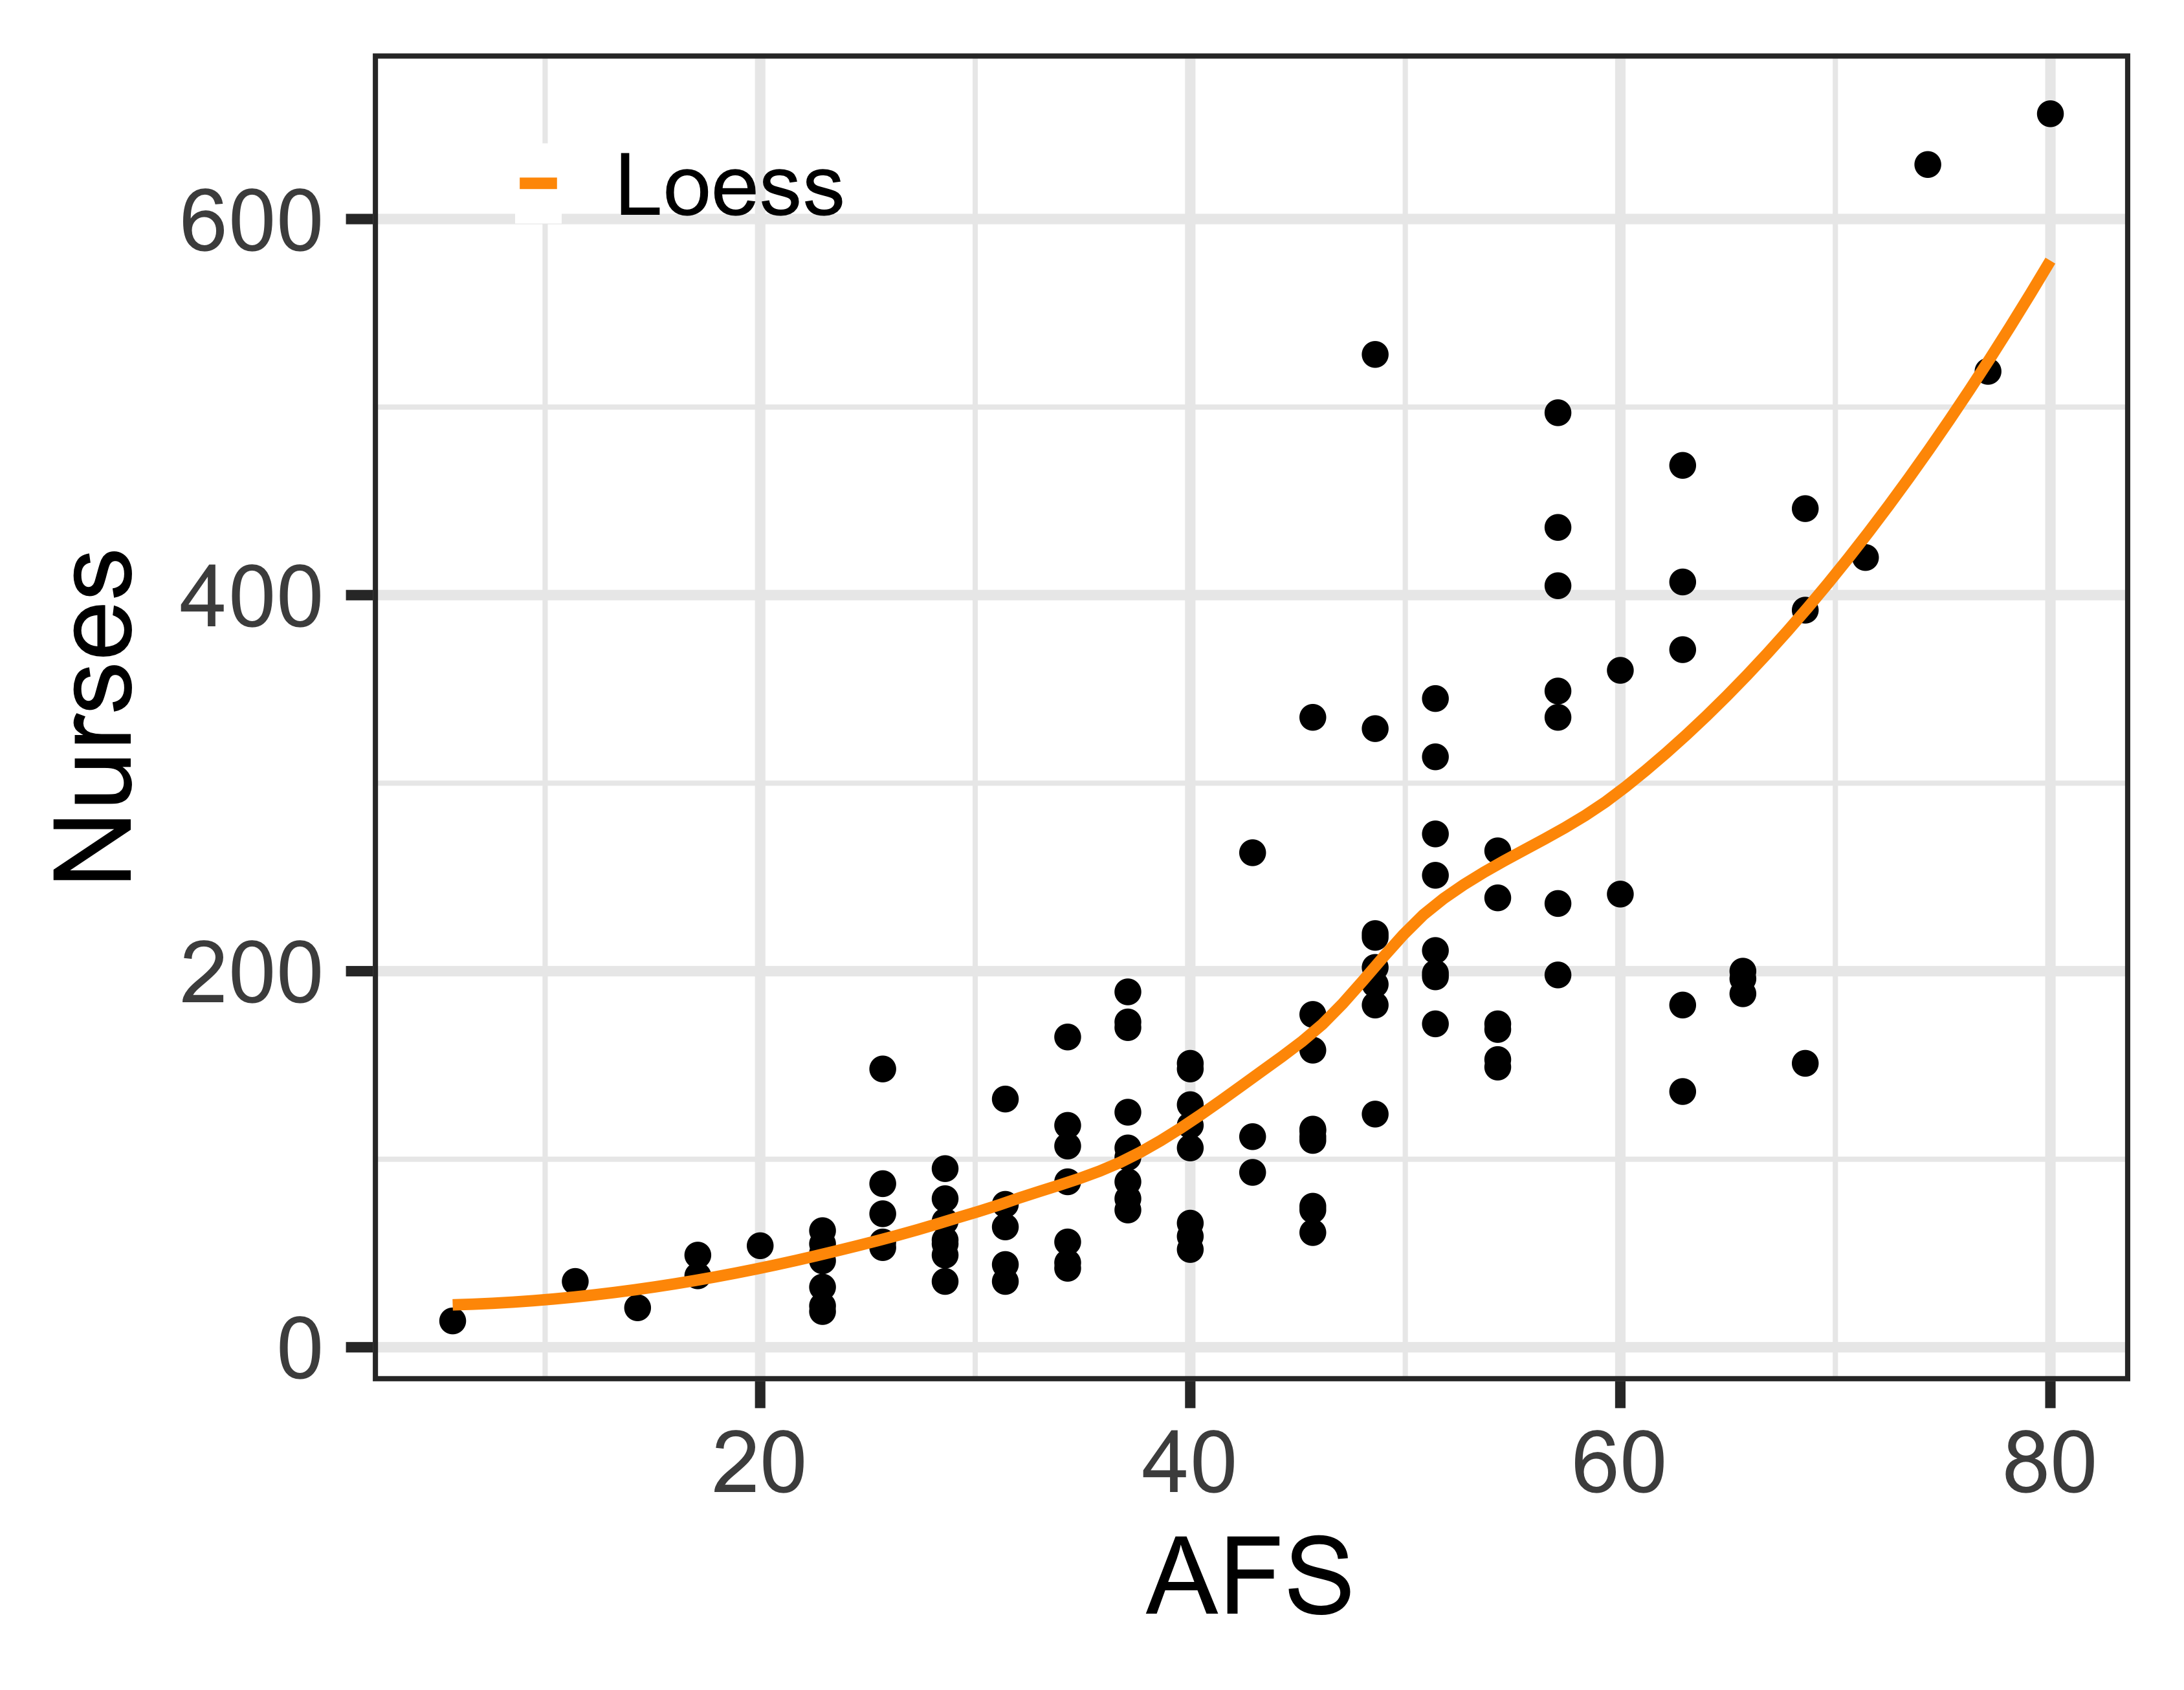
\includegraphics[width = 0.4\textwidth]{img/q01a-single.png}
    \quad
    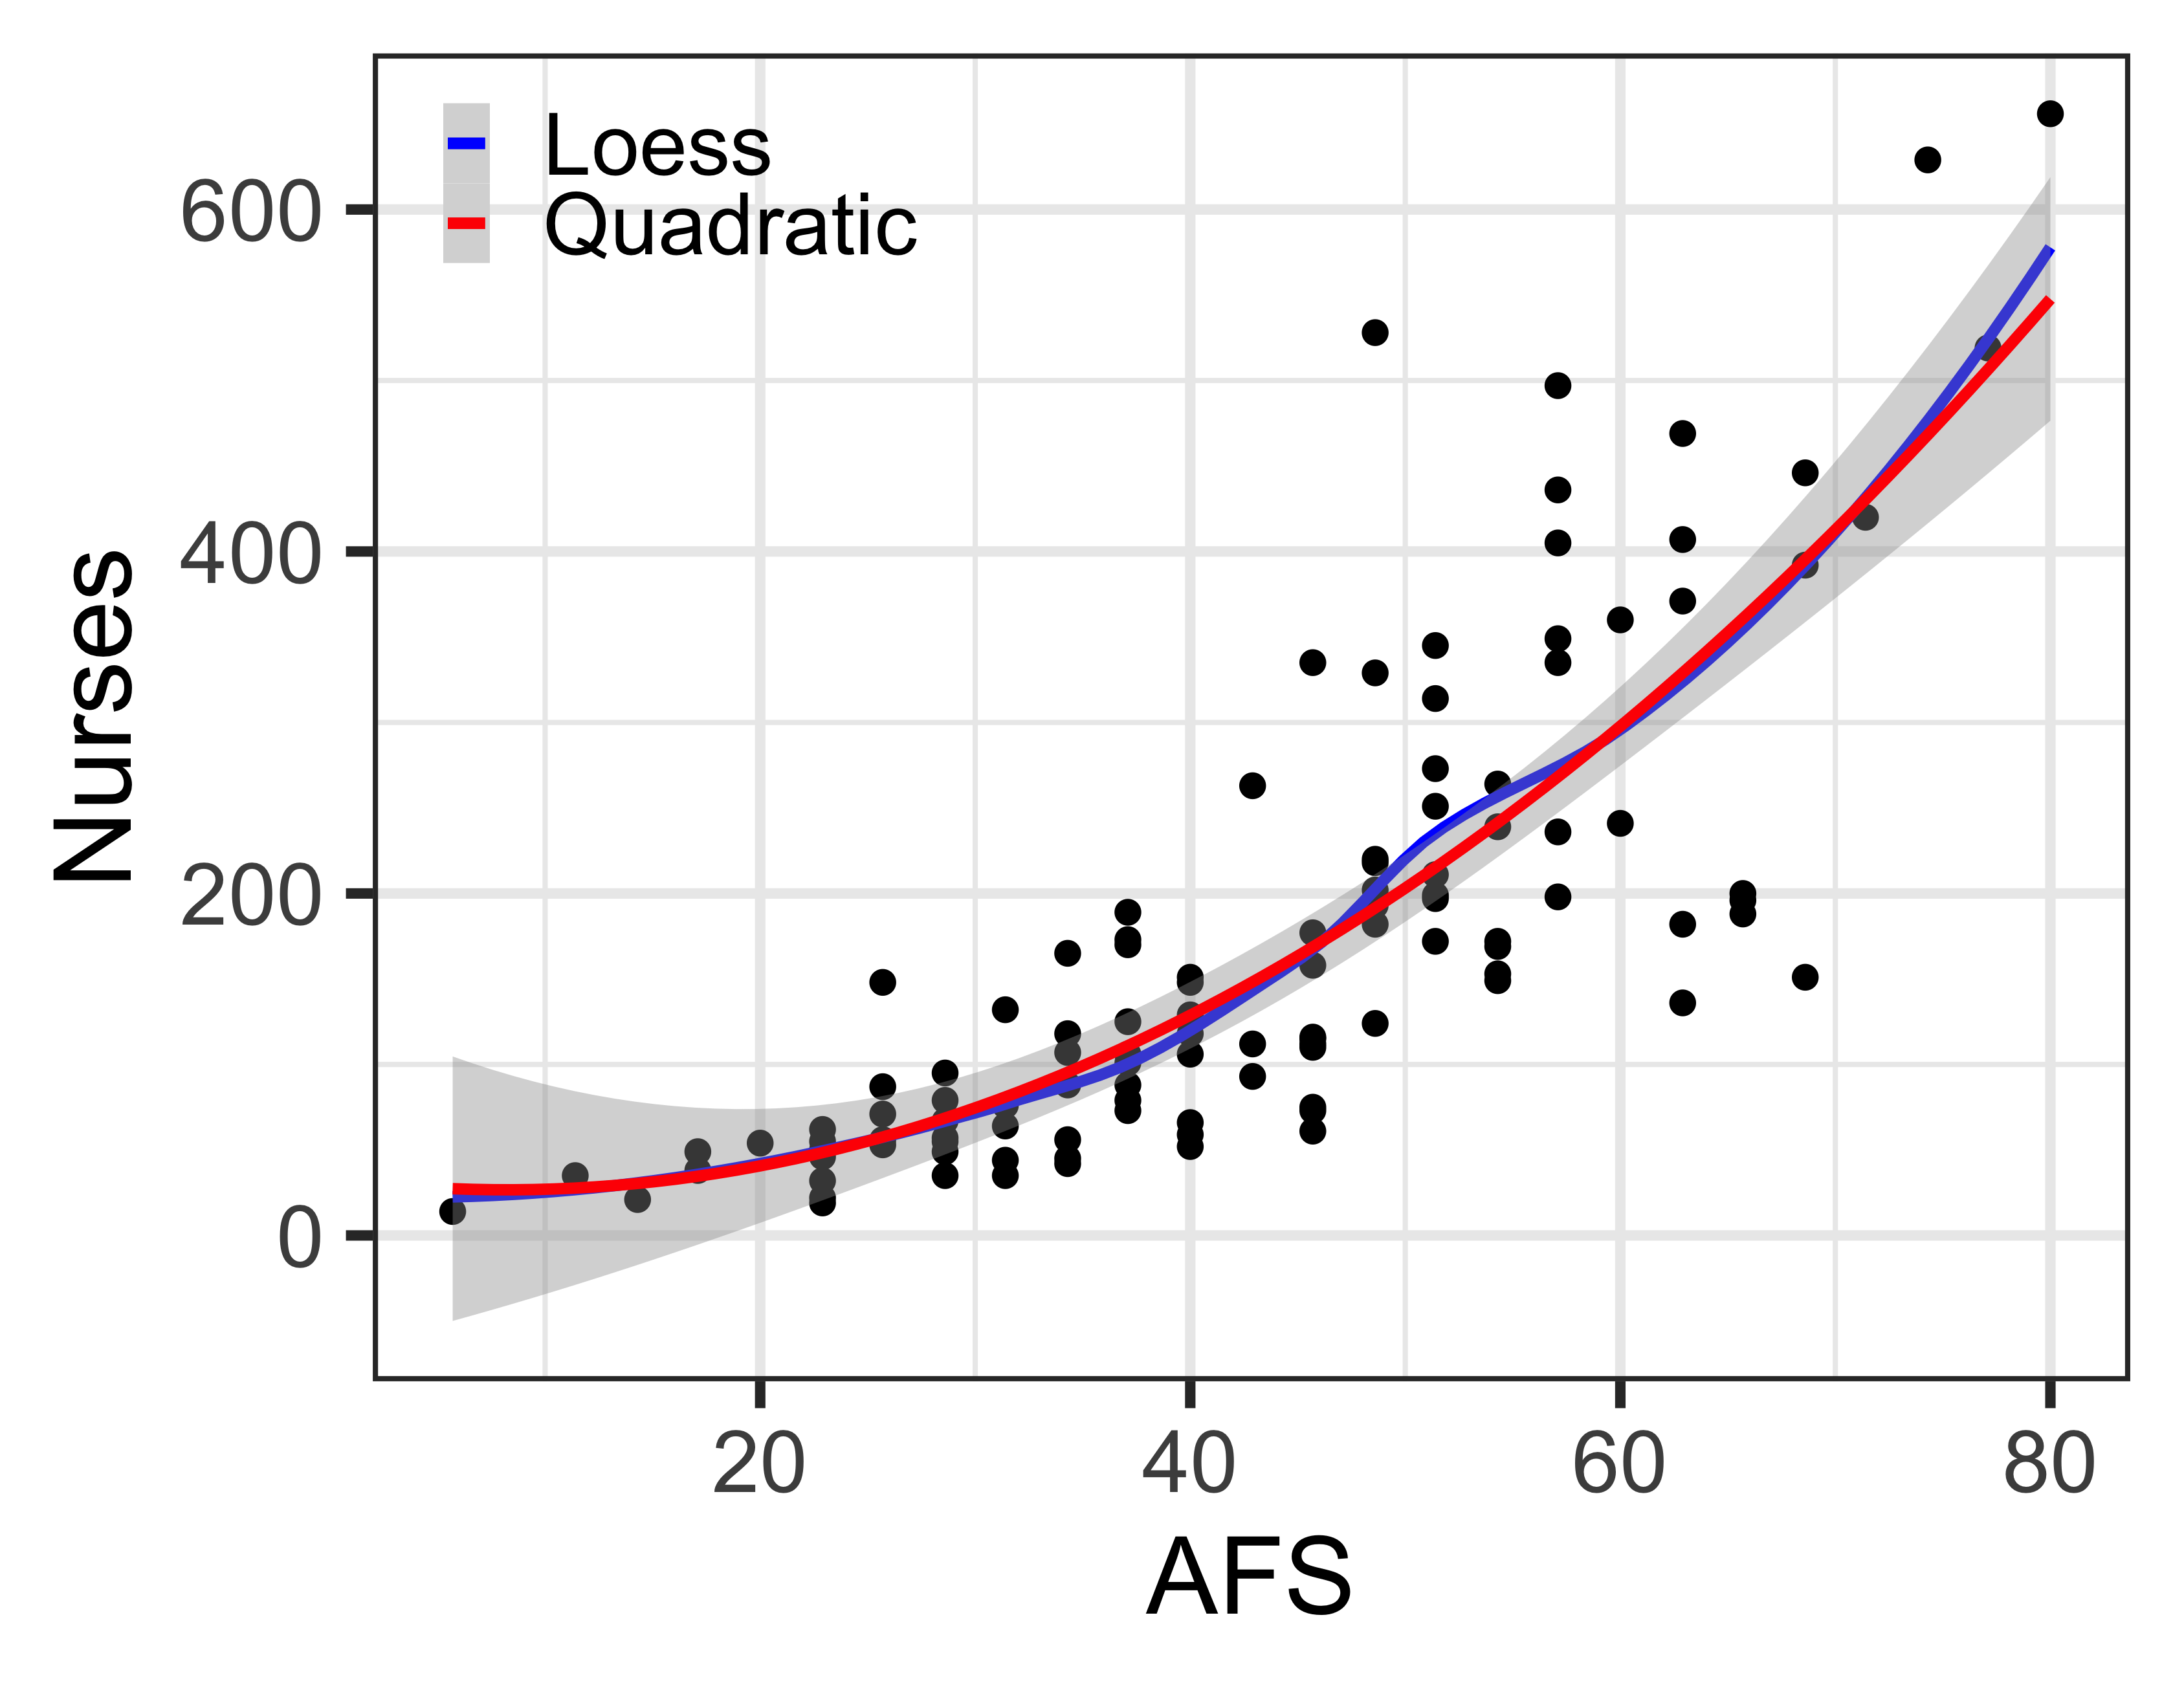
\includegraphics[width = 0.4\textwidth]{img/q01a-both.png}
    \caption{Overlaying a loess smoother and a quadratic polynomial to the scatterplot of AFS vs. Nurses.
    The left plot displays only the loess smoother, while the right plot displays both.}
    \label{fig-q01a}
\end{figure}
\begin{itemize}
    \item[(a)] The loess smoother is the blue line displayed in Figure \ref{fig-q01a}. For clarity, the left plot displays only the loess smoother. The loess 
    smoother indicates that a linear function does not seem plausible for this data, as the curve is too non-linear. 
    \item[(b)] The fitted quadratic model is given by \(\hat{Y} = 33.548 - 1.666 x + 0.101 x^2\), and can be see in the right panel of Figure \ref{fig-q01a}. 
    As we can see, the quadratic model almost perfectly overlays the loess smoother, further indicating that a linear relationship is not plausible. 
    \item[(c)] Given our model \(Y = \beta_0 + \beta_1 X + \beta_2 X^2 + \epsilon\), to determine if the quadratic term can be dropped from the model, we will
    test \(H_0 : \beta_2 = 0\) against \(H_a : \beta_2 \neq 0\). The \(p\)-value for this test is \(0.00032\), so for any reasonable significance level, we
    will reject \(H_0\). It seems that there is a non-negligible quadratic relationship. Interestingly, if one were to re-run the same test for \(\beta_0\) and 
    \(\beta_1\), the corresponding \(p\)-values would be \(0.515\) and \(0.495\), which would not give us grounds to reject either of those null hypotheses.
    That is, we could say the slope and linear term of this model are insignificant, but the quadratic term is not. 
    \item[(d)] When AFS is \(30\%{}\), a \(95\%{}\) prediction interval is \(\big( -89.781, 239.004 \big)\), and when AFS is \(60\%{}\), a \(95\%{}\) prediction 
    interval is \(\big( 133.136, 462.503 \big)\). The simultaneous confidence level for both of these intervals is \(0.95^2 = 0.9025\), so we are \(90.25\%{}\) 
    confident that both of these predictions will occur. 
    \begin{figure}[ht]
        \centering
        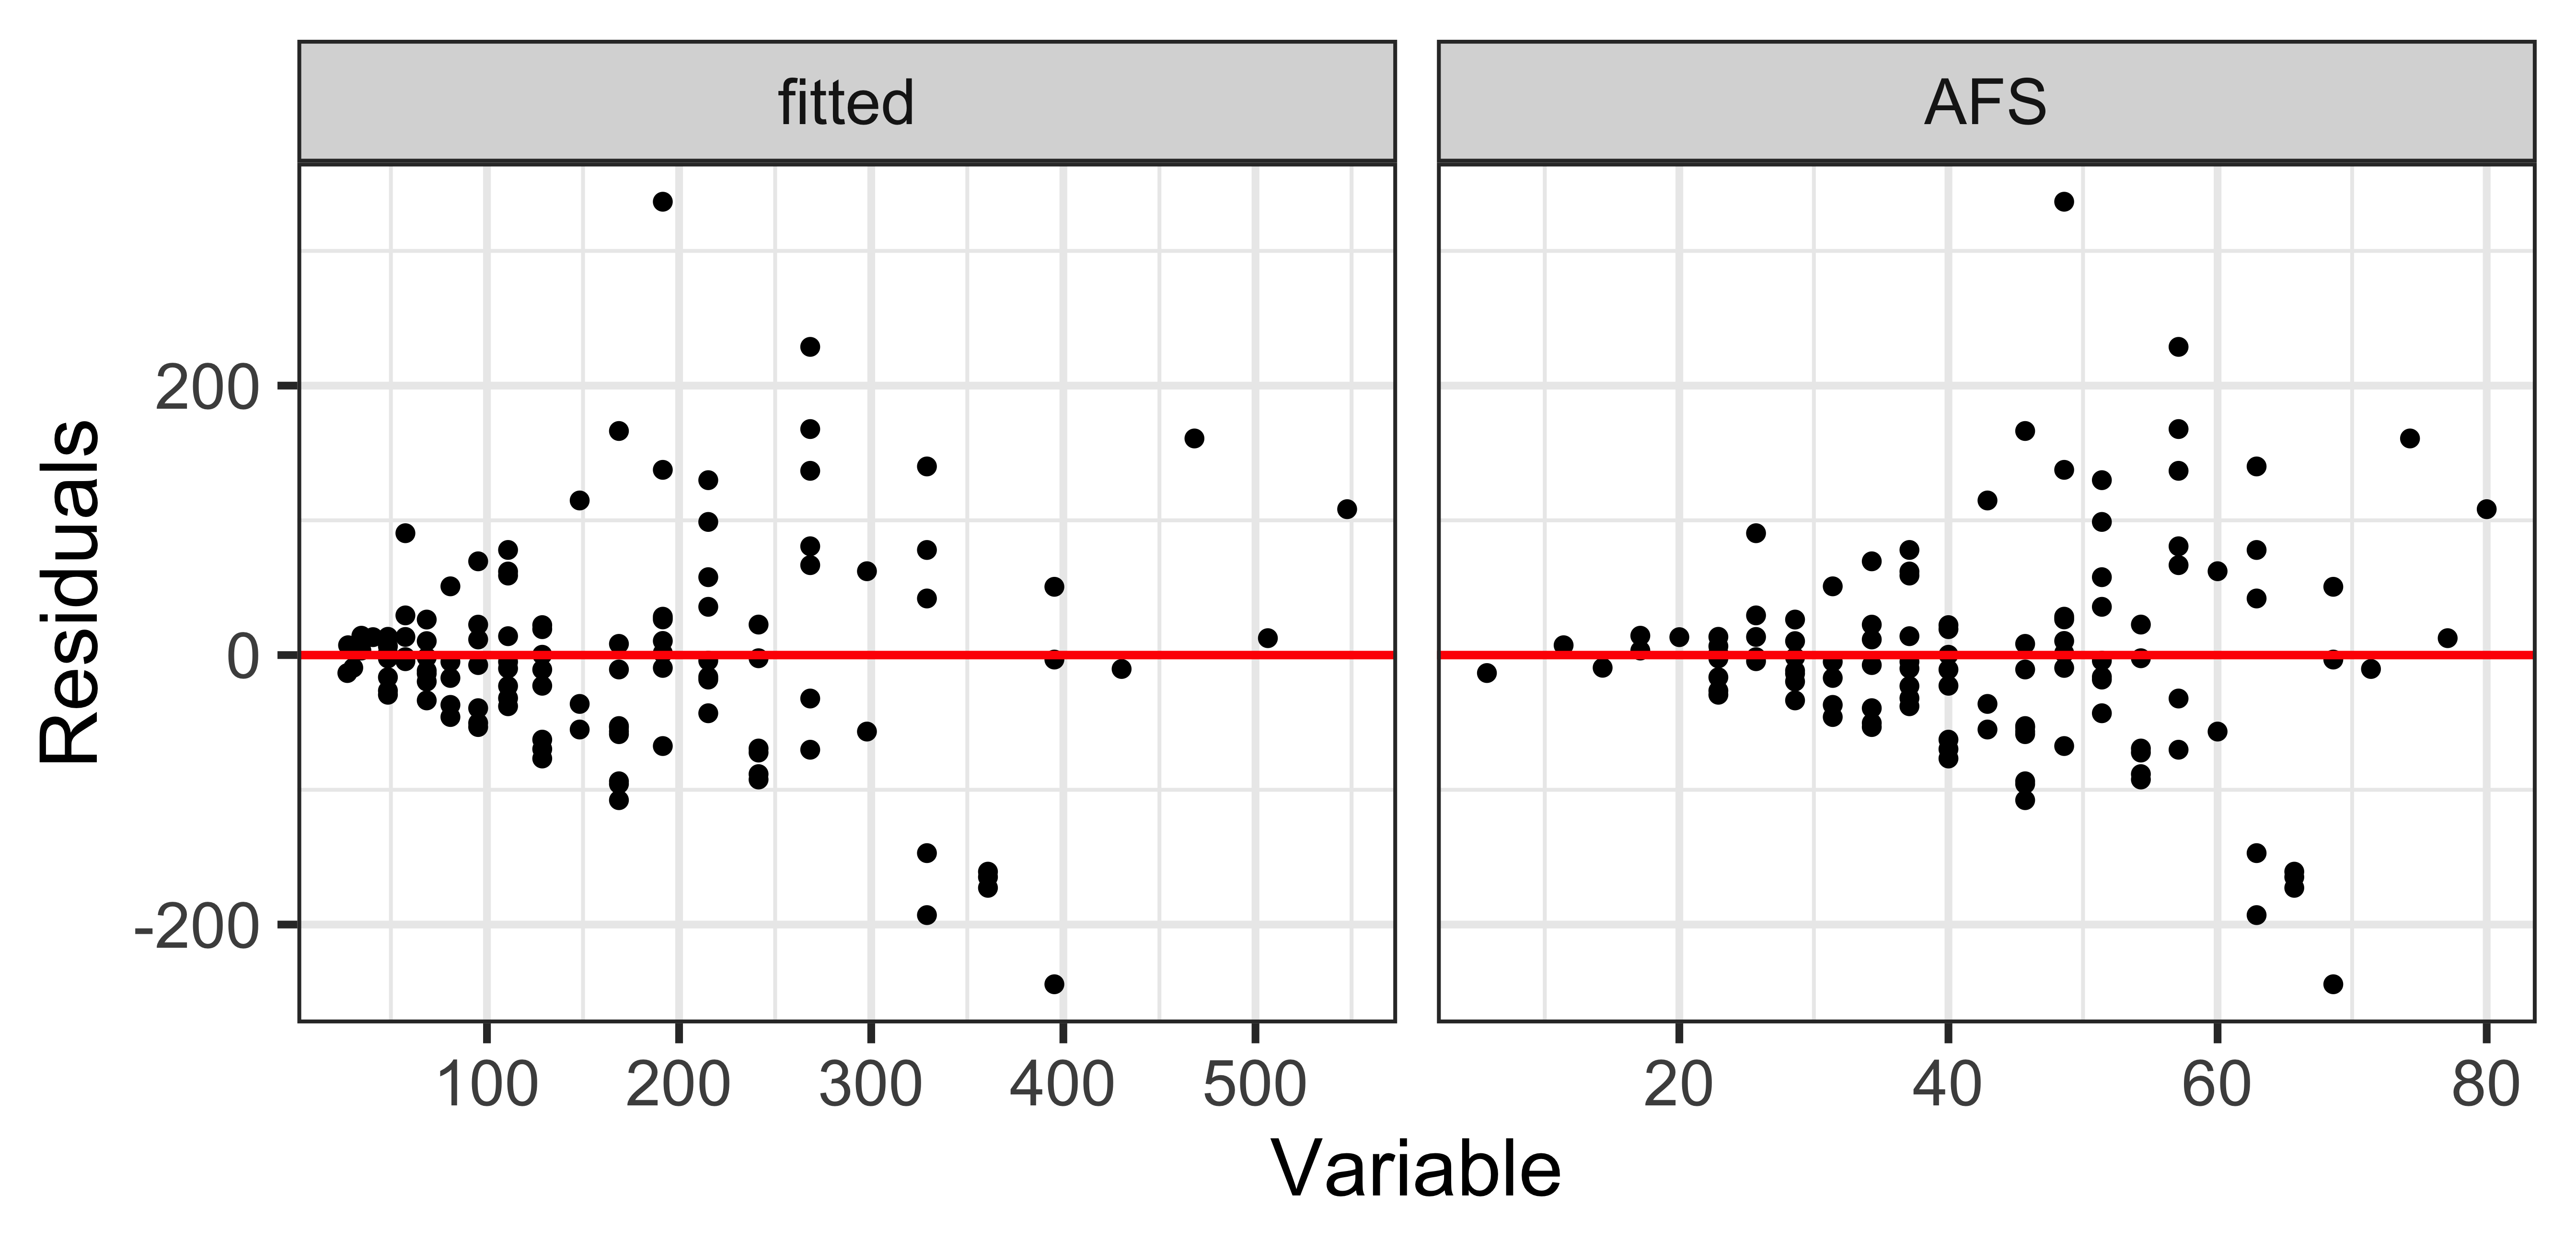
\includegraphics[width = 0.55\textwidth]{img/q01-residuals.png}
        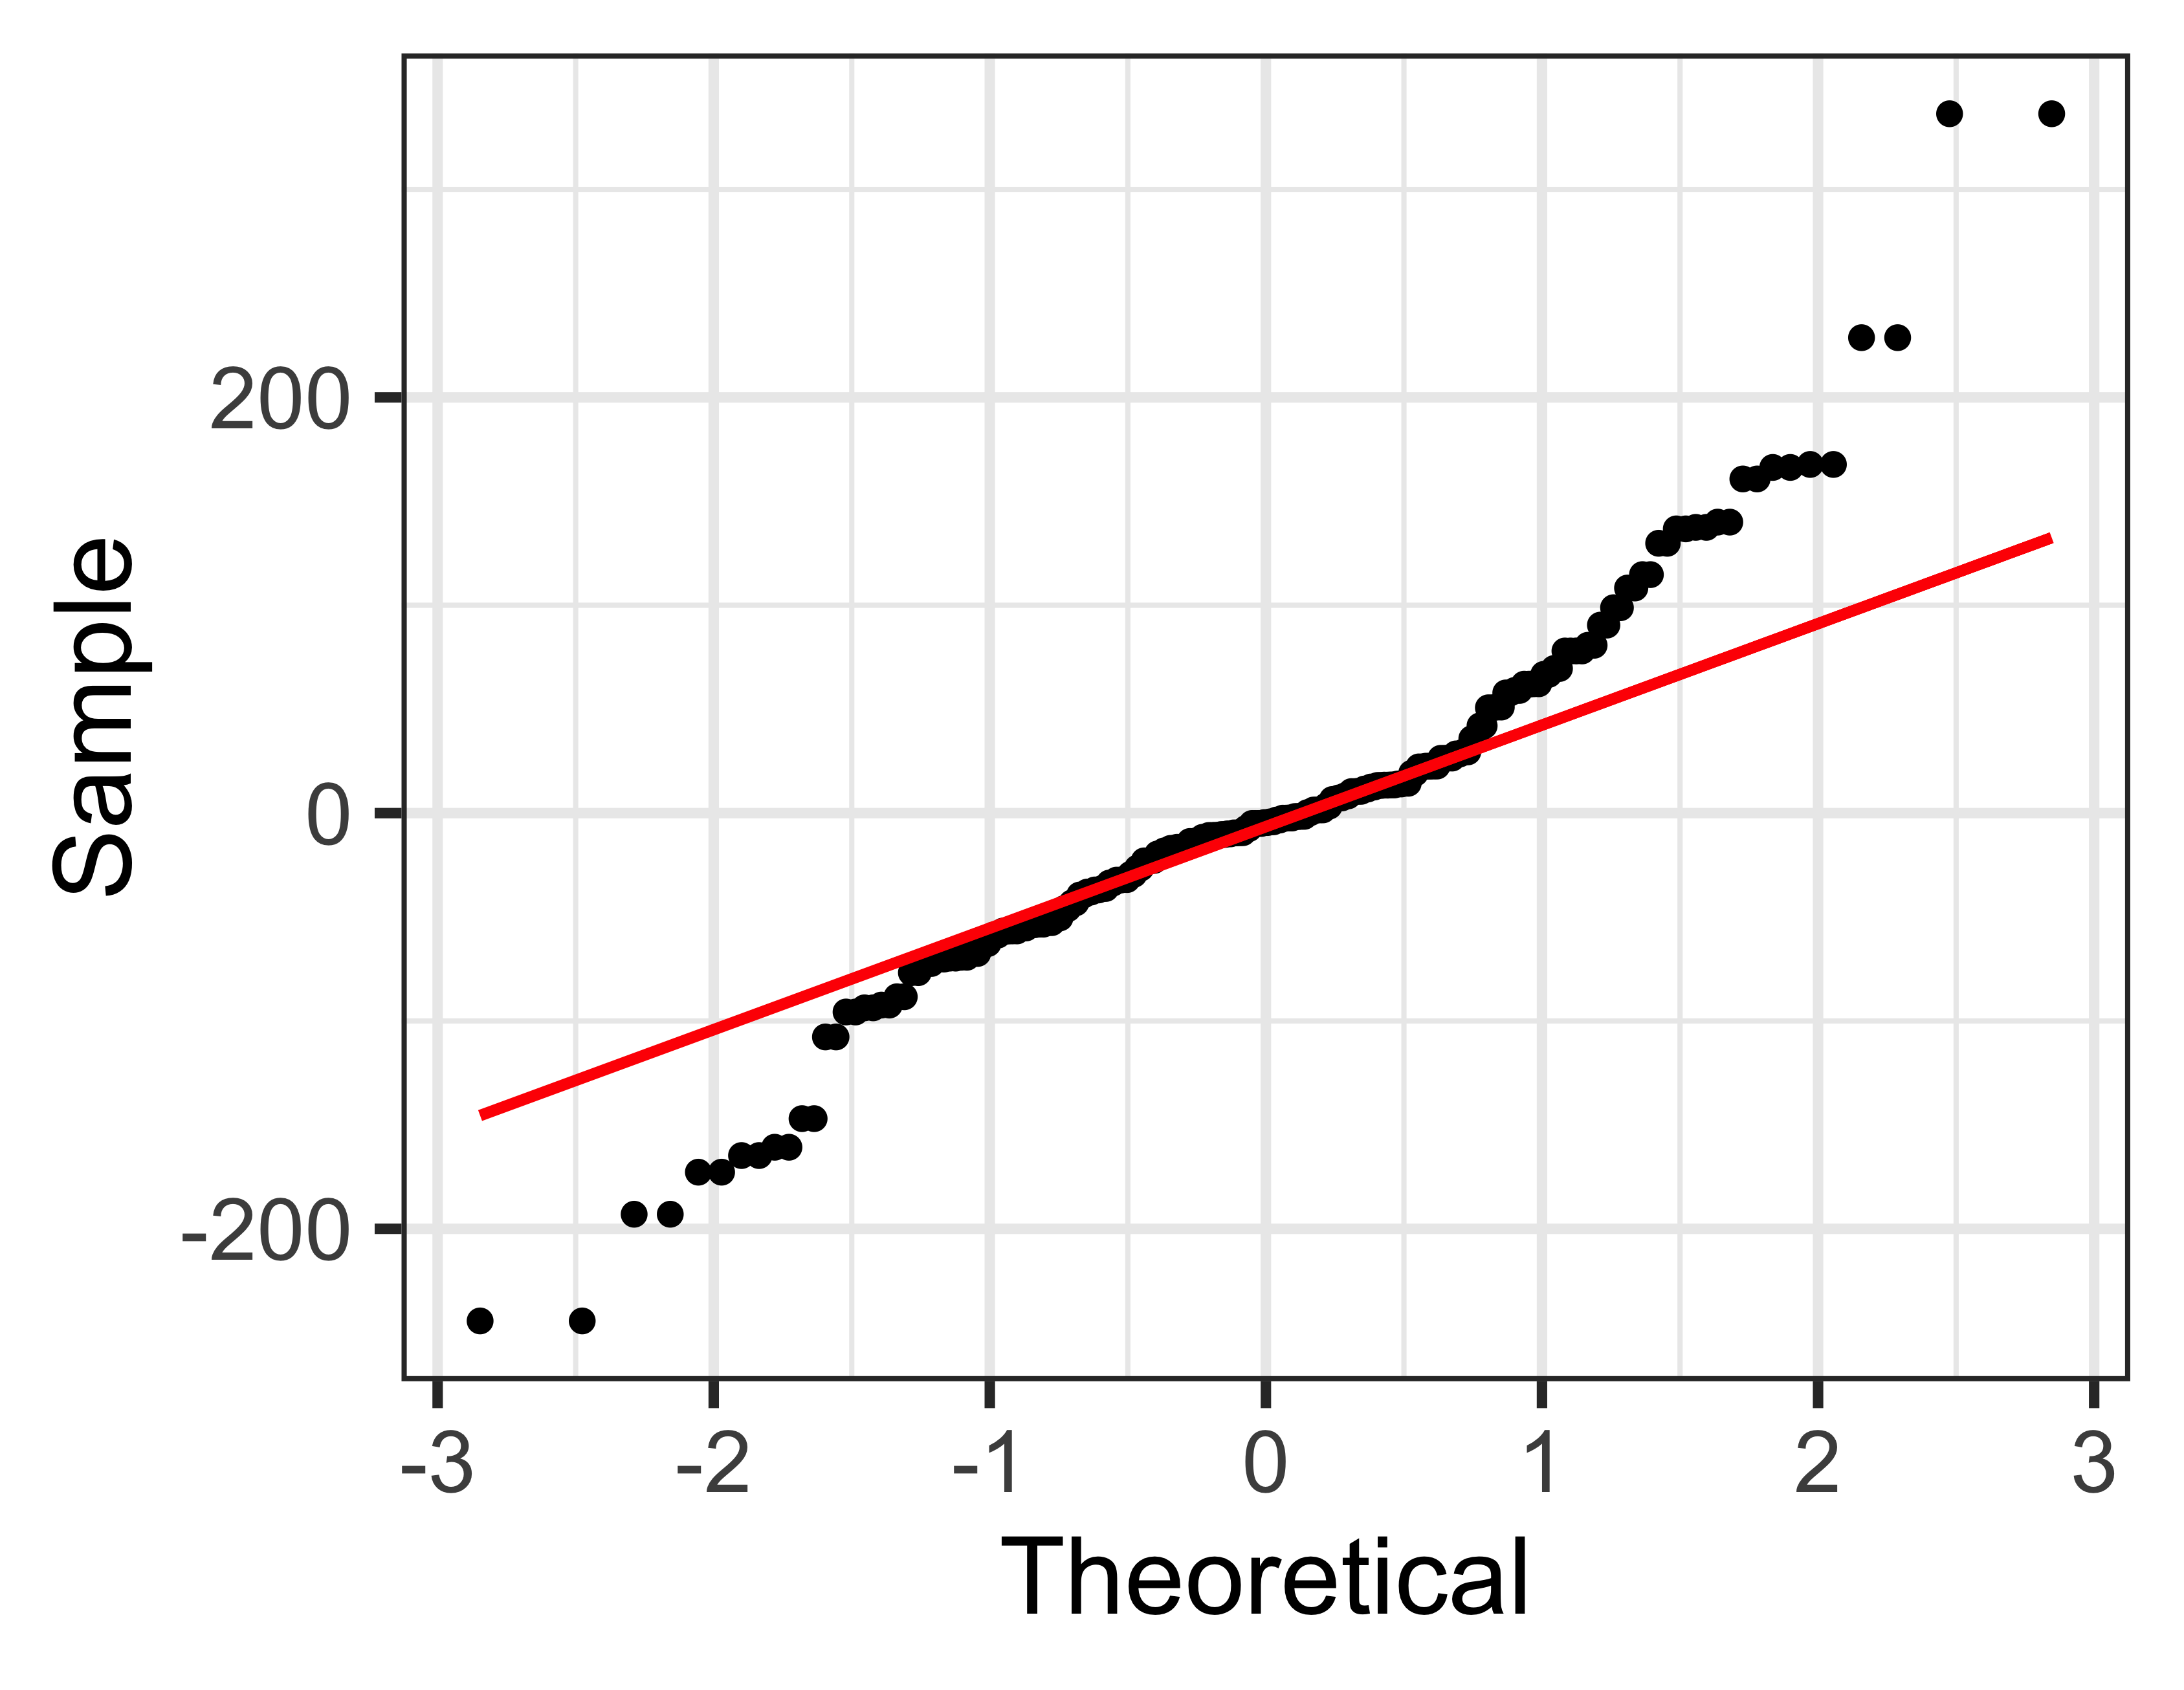
\includegraphics[width = 0.35\textwidth]{img/q01-qqplot.png}
        \caption{Diagnostic plots for the quadratic model.}
        \label{fig-q01-diag}
    \end{figure}
    \item[(e)] The diagnostic plots have been printed in Figure \ref{fig-q01-diag}. We can see right away that the assumption of equal variance among the 
    residuals is violated. For both residual plots, the residuals create a cone-like pattern, where the variance in the residuals starts small, and then 
    increases. In addition, there are several significant outliers in the QQ-plot, meaning that the assumption of normally-distributed residuals is most 
    likely being violated as well. 
\end{itemize}


%' ============================================================================================================================================================
\section{Question 2} \noindent
\mycolaba{None}
\begin{itemize}
    \item[(a)] See the attached \texttt{R} code.
    \item[(b)] The scatterplot matrix can be seen in Figure \ref{fig-q02-corr}. It seems that there is a difference between hospitals with or without 
    a medical school affiliation.
    \begin{figure}[ht]
        \centering
        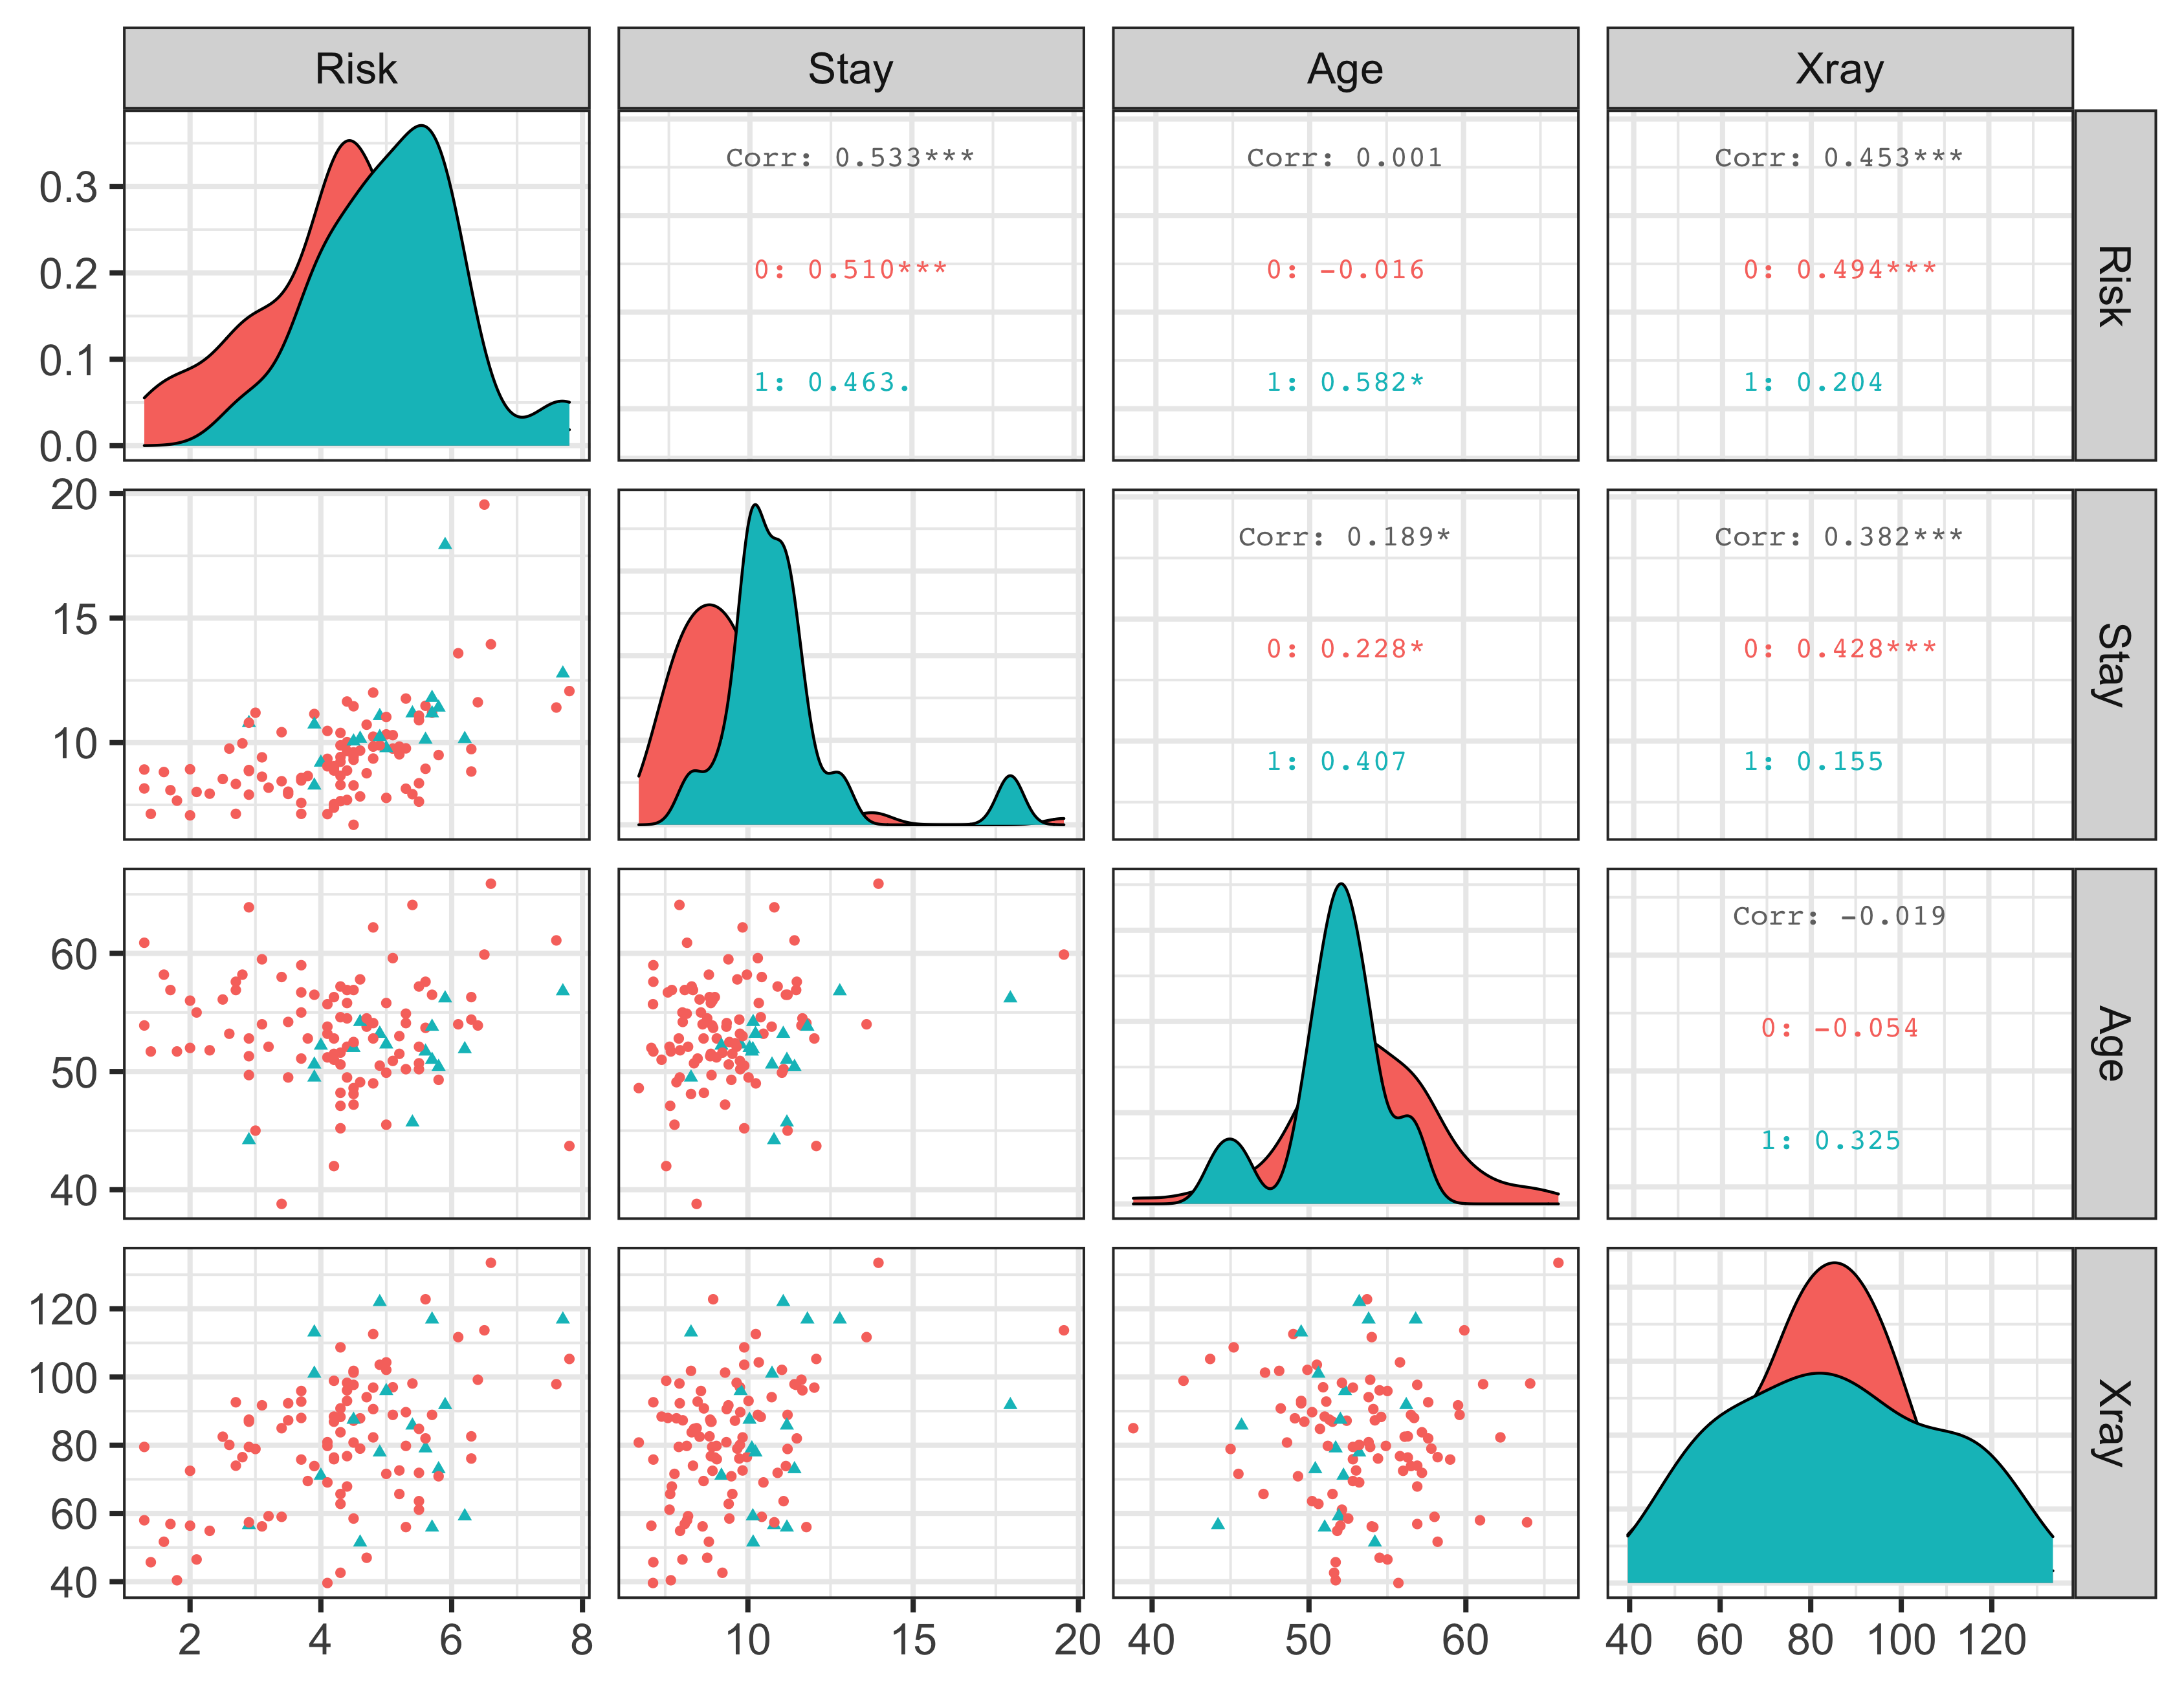
\includegraphics[width = 0.9\textwidth]{img/q02-correlation.png}
        \caption{A scatterplot matrix of Risk against Stay, Age, and Xray. Here, hospitals without a medical school
        affiliation are labeled as red circles, and those with a medical school affiliation are labeled as blue triangles.}
        \label{fig-q02-corr}
    \end{figure}
    \item[(c)] Let \(X_1\), \(X_2\), \(x_3\), and \(X_4\) correspond to Stay, Age, Xray, and MS, respectively. We are considering two models:
    \begin{align}
        Y &= \beta_0 + \beta_1 X_1 + \beta_2 X_2 + \beta_3 X_3 + \beta_4 X_4, \label{mod-no-int}\\
        Y &= \beta_0 + \beta_1 X_1 + \beta_2 X_2 + \beta_3 X_3 + \beta_4 X_4 + \beta_5 X_1 X_4 + \beta_6 X_2 X_4 + \beta_7 X_3 X_4. \label{mod-yes-int}
    \end{align}
    Model (\ref{mod-no-int}) is a linear model with the four predictors, and model (\ref{mod-yes-int}) has the same linear terms plus three interaction terms. 
    For notational ease, let \(\tilde{\bm{\beta}} = (\beta_5, \beta_6, \beta_7)^T\), i.e. \(\tilde{\bm{\beta}}\) is a vector that contains the coefficients of 
    the interaction terms. 
    We want to test that the interaction terms are negligible, so we will test \(H_0: \tilde{\bm{\beta}} = \mathbf{0}\) against 
    \(H_a : \tilde{\bm{\beta}} \neq \mathbf{0}\).
    Using \texttt{R}, we can easily fit a linear model both with and without interactions. In addition, we can conduct an F-test to get a 
    \(p\)-value of \(0.1539\), so we fail to reject the null hypothesis. The data seems to indicate that the interaction terms are 
    negligible in the model. 
    \item[(d)] Using model (\ref{mod-no-int}), a \(95\%{}\) confidence interval for \(\beta_4\) is \(\big( -0.320, 0.896 \big)\). Since zero is withing this 
    confidence interval, we can conclude that the effect of medical school affiliation is negligible in this model. 
\end{itemize}


%' ============================================================================================================================================================
\section{Question 3} \noindent
\mycolaba{None}
\begin{itemize}
    \item[(a)] A scatterplot matrix has been printed in Figure \ref{fig-q03-corr}.
    \begin{figure}[ht]
        \centering
        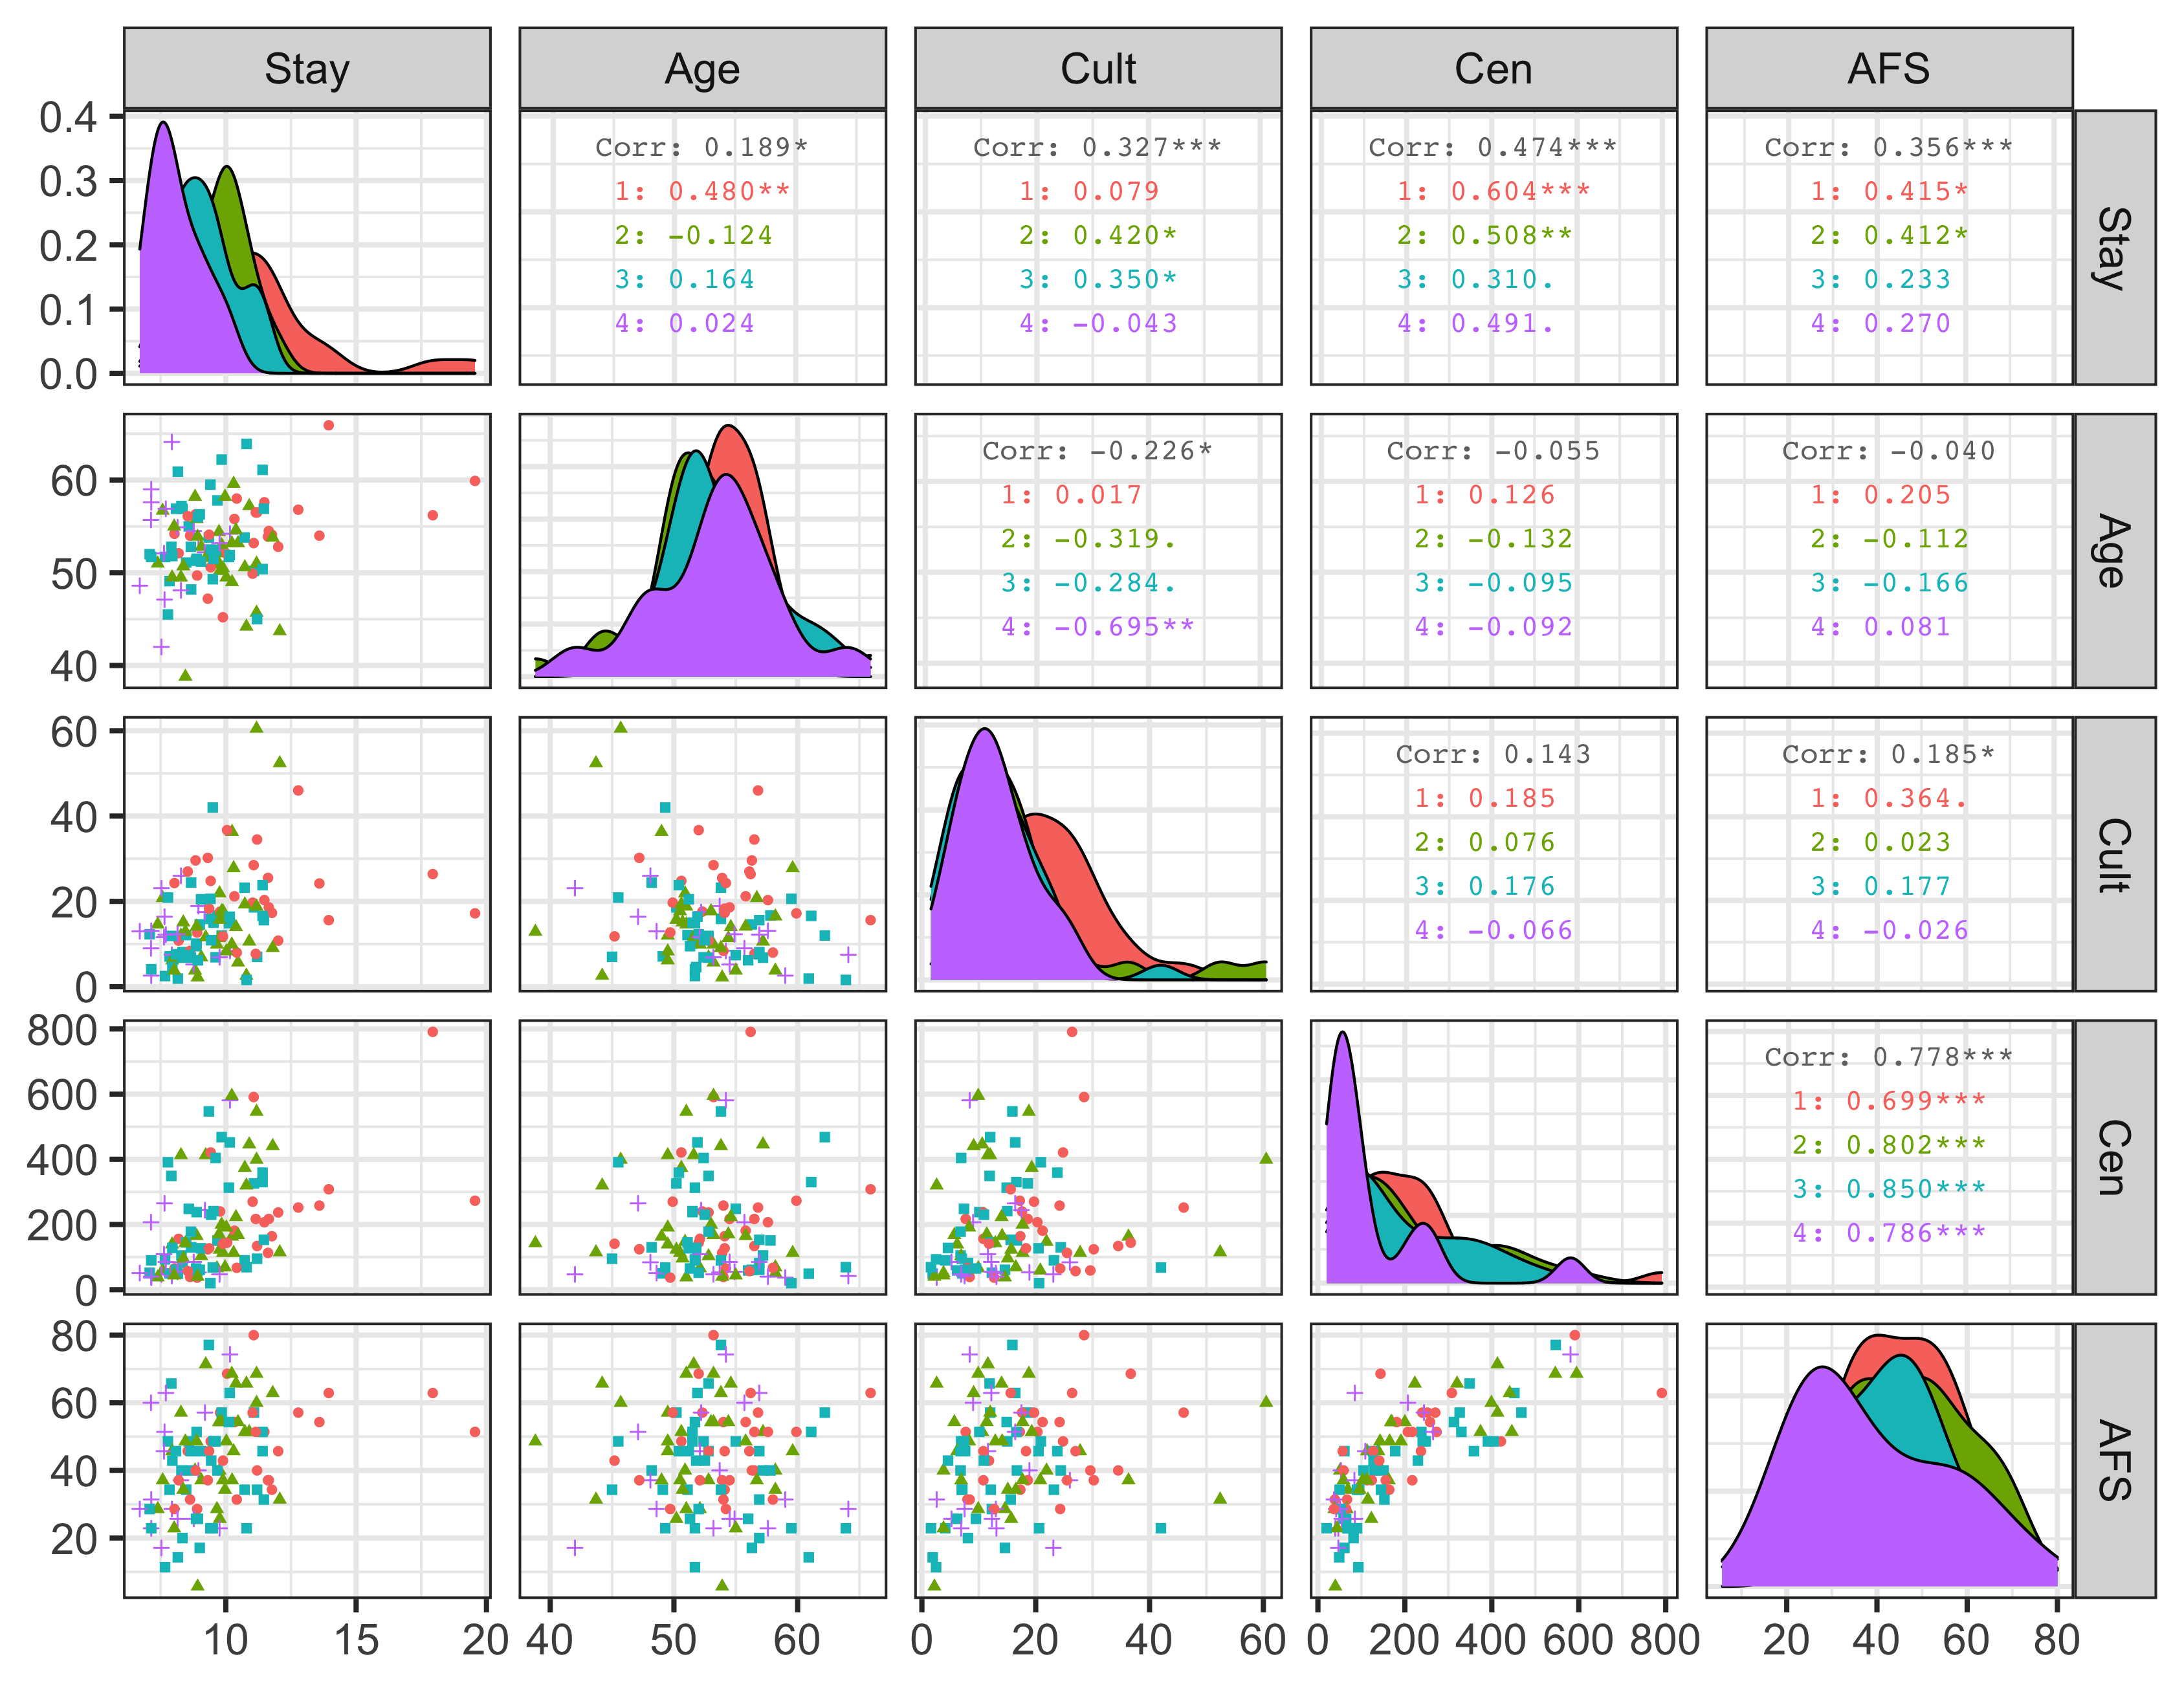
\includegraphics[width = 0.9\textwidth]{img/q03-correlation.png}
        \caption{A scatterplot matrix of Stay against Age, Cult, Cen, and AFS.}
        \label{fig-q03-corr}
    \end{figure}
    \item[(b)] Let \(X_1, \ldots, X_4\) denote Age, Cult, Cen, and AFS, respectively. Our four linear models are given by 
    \begin{subequations}
        \begin{align}
            \hat{Y} &= 4.198 + 0.104 X_1 + 0.0403 X_2 + 0.00660 X_3 - 0.0208 X_4 \label{mod-reg01} \\
            \hat{Y} &= 3.238 + 0.104 X_1 + 0.0403 X_2 + 0.00660 X_3 - 0.0208 X_4 \label{mod-reg02} \\
            \hat{Y} &= 2.681 + 0.104 X_1 + 0.0403 X_2 + 0.00660 X_3 - 0.0208 X_4 \label{mod-reg03} \\
            \hat{Y} &= 2.048 + 0.104 X_1 + 0.0403 X_2 + 0.00660 X_3 - 0.0208 X_4 \label{mod-reg04}
        \end{align}
    \end{subequations}
    Model (\ref{mod-reg01}) is for when we are in region 1, (\ref{mod-reg02}) for region 2, and so on. 
    \item[(c)] From our four models, we have \(\hat{\beta}_2 = 0.0403\). A \(99\%{}\) confidence interval for \(\beta_2\) is 
    \(\big( 0.00278, 0.0778 \big)\). 
    \item[(d)] We can alternatively write our four separate estimated models as a single model using indicator functions. Let 
    \(X_5 = \mathbb{I}(\text{Region} = 2)\), \(X_6 = \mathbb{I}(\text{Region} = 3)\), and \(X_7 = \mathbb{I}(\text{Region} = 4)\).
    Then our linear function takes the form 
    \begin{align}
        Y = \beta_0 + \sum_{i = 1}^7 \beta_i X_i \label{mod-region-whole}
    \end{align}
    In this form, the estimated model parameters are given by \(\hat{\beta}_0 = 4.198\), \(\hat{\beta}_5 = - 0.960\), \(\hat{\beta)}_6 = -1.517\), and 
    \(\hat{\beta}_7 = -2.150\). Letting \(\tilde{\bm{\beta}} = (\beta_5, \beta_6, \beta_7)^T\), if we want to test whether or not the average stay does not 
    depend on the region, we will test \(H_0 : \tilde{\bm{\beta}} = \mathbf{0}\) against \(H_a : \tilde{\bm{\beta}} \neq \mathbf{0}\). One method to test this 
    is to fit a reduced model without accounting for region, and then fitting an anova model between the two. Doing this, we have a \(p\)-value of 
    \(3.77 \times 10^{-5}\), so for any reasonable significance level we will reject \(H_0\). The data seems to indicate that the geographic region does play 
    a significant role in average patient stay. 
\end{itemize}


%' ============================================================================================================================================================
\section{Question 4} \noindent
\mycolaba{None}
\begin{itemize}
    \item[(a)] For this question we will assume the matrix \(\mathbf{X}\) is \textsl{centered}, so that each predictor has mean zero. 
    In \(n\)-dimensional Euclidean vector space, for any \(\mathbf{v} \in \mathbb{R}^n\) we have \(\|\mathbf{v}\|^2 = \mathbf{v}^T\mathbf{v}\), 
    so the ridge regression loss function becomes 
    \begin{align*}
        Q(\bm{\beta}; \lambda) 
        = \| \mathbf{y} - \mathbf{X}\bm{\beta} \|^2 + \lambda \|\bm{\beta}\|^2
        = \mathbf{y}^T\mathbf{y} - 2 \bm{\beta}\mathbf{X}^T\mathbf{y} + \bm{\beta} \mathbf{X}^T \mathbf{X} \bm{\beta} + \lambda \bm{\beta}^T \bm{\beta}.
    \end{align*}
    Differentiating the loss function with respect to \(\bm{\beta}\) gives us 
    \begin{align*}
        \frac{\partial Q}{\partial \bm{\beta}}
        = -2 \mathbf{X}^T \mathbf{y} + 2 \mathbf{X}^T\mathbf{X}\bm{\beta} + 2 \lambda \bm{\beta}
        = -2 \mathbf{X}^T \mathbf{y} + 2 \big( \mathbf{X}^T\mathbf{X} + \lambda \mathbf{I} \big) \bm{\beta}
        \overset{\text{set}}{=} \mathbf{0},
    \end{align*}
    and finally solving for \(\bm{\beta}\) gives us 
    \(\hat{\bm{\beta}}_{\lambda} = \big( \mathbf{X}^T\mathbf{X} + \lambda \mathbf{I} \big)^{-1} \mathbf{X}^T\mathbf{y}\).
    \item[(b)] When \(\lambda = 0\) we have \(\hat{\bm{\beta}}_{\lambda = 0} = \big( \mathbf{X}^T\mathbf{X} \big)^{-1} \mathbf{X}^T\mathbf{y}\), the OLS 
    estimator. 
\end{itemize}

\end{document}